\input{../header}
\usepackage{pgfplots}
\usepackage{tabularx}
\newcolumntype{Y}{>{\centering\arraybackslash}X}

\everymath{\displaystyle}
\begin{document}
%

\newcommand{\axesandchart}{
\begin{minipage}{0.5\textwidth-1em}
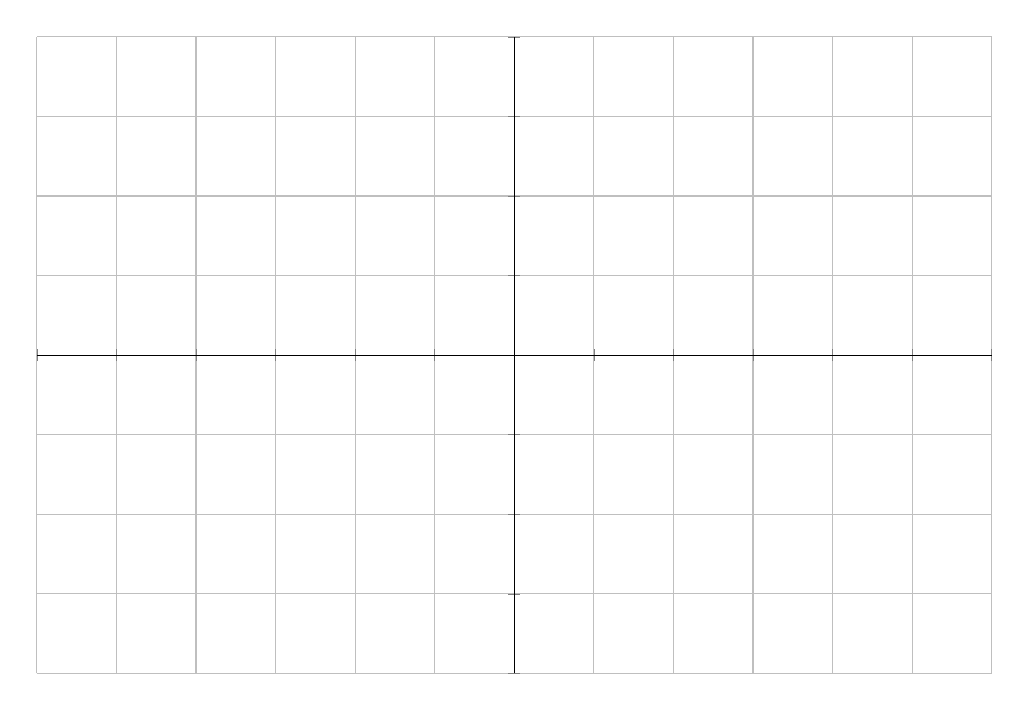
\begin{tikzpicture}
    \begin{axis}[
        grid = both,
        xmin=-6, xmax=6, xtick distance = 1, xticklabels={},
        ymin=-4, ymax=4, ytick distance = 1, yticklabels={},
        axis x line = middle, x axis line style = -,
        axis y line = middle, y axis line style = -,
        axis equal image,
        scale only axis,
        width = \textwidth
    ] 
    \end{axis}
\end{tikzpicture}

\vspace{5ex}

\begin{tikzpicture}
    \begin{axis}[
        % center the x axis
        axis x line=middle, x axis line style = -,
        % we don't need a y axis line ...
        axis y line=none,
        % ... and thus there is no need for much `height' of the axis
        height=50pt,
        xmin=-6, xmax=6, xtick distance = 1, xticklabels={},
        ymin=-0.5, ymax=0.5,
        axis equal image,
        scale only axis,
        width = \textwidth
    ]
    \end{axis}
    
\end{tikzpicture}
\end{minipage}
}

%\onehalfspacing
\allowdisplaybreaks
%##################################################################
\section{Highest and lowest points}

For each of the graphs below:
\begin{enumerate}[leftmargin=0pt]
    \item Mark the very highest point and the very lowest point of $f(x)$.
    \item Mark any points that are ``locally'' the highest or lowest.
    \item On the number line below the graph, mark any $x$-values where $f'(x)$ would equal $0$.
    \item On the number line below the graph, mark any $x$-values where $f'(x)$ would not exist.
    \item On the number line below the graph, highlight the intervals where $f'(x) < 0$.
    \item In a different color, highlight the intervals where $f'(x) > 0$.
\end{enumerate}

\axesandchart \hfill 
\axesandchart

\vfill

\axesandchart \hfill
\axesandchart

\pagebreak

\axesandchart \hfill 
\axesandchart

\vfill

\axesandchart \hfill
\axesandchart

\vfill

Now some questions for you:
\begin{enumerate}
    \item What connections do you see between the highest and lowest points you marked on the graph and the locations you marked on the number line?
    \item What connections do you see between the highlights you made on the number line and the $x$-values where either $f'(x) = 0$ or $f'(x)$ does not exist?
    \item Which blank boxes can you fill in in the table below?
\end{enumerate}
\def\arraystretch{1.5}
\begin{tabularx}{\textwidth}{|c|Y|Y|Y|Y|Y|Y|}\hline
    $f(x)$   & Positive & Negative &          &          &          &          \\\hline 
    $f'(x)$  &          &          & Positive & Negative &          &          \\\hline 
    $f''(x)$ &          &          &          &          & Positive & Negative \\\hline
\end{tabularx}

\end{document}